%%%%%%%%%%%%%%%%%%%%%%%%%%%%%%%%%%%%%%%%%%%%%%%%%%%%%%%%%%%%%%%%%%%
%%% Den här mallen är skriven av Magnus Gustafsson (MG),
%%% tillämpad fysik, Luleå tekniska universitet. 
%%% Den är baserad på TVM:s rapport-mall/guide i word och
%%% Lars-Göran Westerbergs latex-mall som använts i kurserna
%%% Ingenjörsvetenskap, och Ingenjörsvetenskap och rymdteknik.
%%% Erik Elfgren har också bidragit med en del förbättringar.
%%% Om du har kommentarer eller önskemål kan du kontakta MG.
%%%%%%%%%%%%%%%%%%%%%%%%%%%%%%%%%%%%%%%%%%%%%%%%%%%%%%%%%%%%%%%%%%%

%%%%%%%%%%%%%%%%%%%%%%%%%%%%%%%%%%%%%%%%%%%%%%%%%%%%%%%%%%%%%
%%%%%%%%%%%%%%%%%%%%%%%%%%%%%%%%%%%%%%%%%%%%%%%%%%%%%%%%%%%%%
% -                  PREAMBLE STARTS HERE                 - %
%%%%%%%%%%%%%%%%%%%%%%%%%%%%%%%%%%%%%%%%%%%%%%%%%%%%%%%%%%%%%
%%%%%%%%%%%%%%%%%%%%%%%%%%%%%%%%%%%%%%%%%%%%%%%%%%%%%%%%%%%%%
%- The preamble defines the formatting of the document.

% - What is written behind the percent mark is not regarded as code. In other words, we use it to comment the code.

\documentclass[a4paper]{article}
\usepackage[margin=1.5cm]{geometry} % Change the margins
\usepackage[utf8]{inputenc} % - Defines what coding LaTeX uses. Use this one.
\usepackage[swedish]{babel}
\usepackage[T1]{fontenc}
\usepackage{graphicx} % - Package for including images in the document.
\usepackage{amsmath}
\usepackage{mathtools}
\usepackage{caption} % Correct spacing for captions
\usepackage{siunitx} % Package for handling numbers (ex \num{1e6}), units (ex \SI{15,3}{Nm}) and intervals (ex \SIrange{10}{20}{\celcius}) correctly
\sisetup{output-decimal-marker={,},range-phrase=--,range-units=single,exponent-product=\cdot} % If you write in English, remove output-marker...
\graphicspath{ {Images/} } % - Path to where the images are located on your computer. In this case I have a folder (look to the left) "Images" where the images are gathered.
\usepackage{hyperref} % - Package for including hyperlinks in the document.
\hypersetup{
  bookmarksopen=true,
  bookmarksopenlevel=0,
  linkcolor={black},
}
%\usepackage[backend=bibtex,style=numeric,bibencoding=ascii]{biblatex} % numeriska referenser
\usepackage[style=apa,backend=biber]{biblatex} % APA-referenser
\DeclareLanguageMapping{swedish}{swedish-apa}  % APA-referenser
 % - Package for the bibliography ("referenser").
\addbibresource{references.bib} % - From where, i.e. which file, the references are taken. The bibliography file is called name.bib; see left column.


% - Can be good to structure the .tex file by dividing the document using commenting. For longer documents you can create separate .tex files for each section and then include these using \import(filename.tex). For the exercise in this course it is suggested that you write everything in this main.tex file. You can of course try using \import if you like. - %

%%%%%%%%%%%%%%%%%%%%%%%%%%%%%%%%%%%%%%%%%%%%%%%%%%%%%%%%%%%%%%
% -               Title and affiliation                    - %
%%%%%%%%%%%%%%%%%%%%%%%%%%%%%%%%%%%%%%%%%%%%%%%%%%%%%%%%%%%%%%

\title{Lathund för rapportskrivning:\\
\LaTeX -mall}

\author{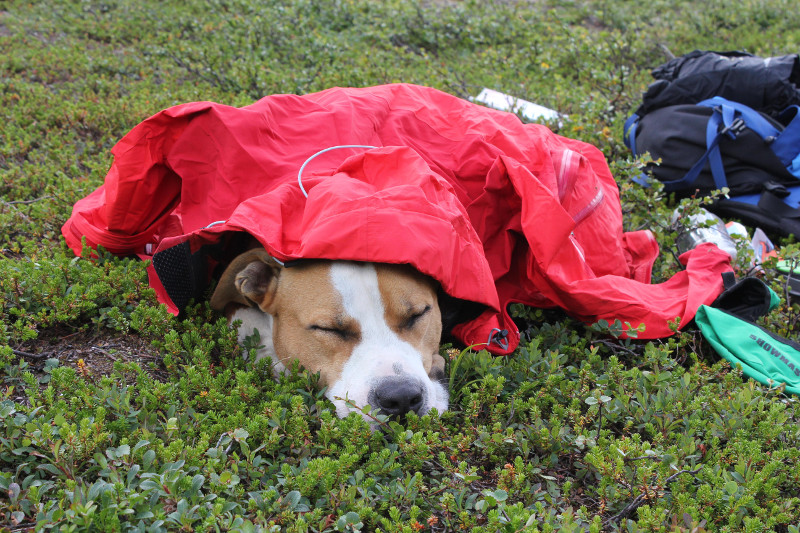
\includegraphics[width=0.6\textwidth]{hund_liten.jpg} \\ \\ \\
Författare \\
{\tt forfattare@student.ltu.se} \\
Institutionen för teknikvetenskap och matematik \\ \\

\includegraphics[width=0.2\textwidth]{ltu_swe.jpg}}
% MG: Bilder på första sidan är bäst att lägga i "author"-
% kommandot såvitt jag kan se.

% Ange författare, e-post samt datum för publiceringen.
% Titelsidan kan också innehålla en figur för att locka läsaren att läsa rapporten.
% Figurens innehåll måste naturligtvis vara kopplat till arbetet som beskrivs i rapporten.
%
% På en titel kan man ställa höga krav. Titeln skall vara klar och beskrivande och fungera
% som en miniatyr-sammanfattning av arbetet. Läsaren skall förstå vad rapporten handlar om
% genom att läsa titeln. Trots det ska titeln vara kort, 4-12 ord, och får inte innehålla
% några formler, förkortningar eller speciella symboler.
%
% En bra titel är en titel som med minsta möjliga antal ord korrekt beskriver innehållet i
% rapporten. Det kan ibland vara praktiskt att ha en titel och en undertitel.
%
% För laborationsrapporter; E-post samt laborationshandledare skall infogas.
%
% Byt LTU logga vid engelsk rapport.

\date{\today}

\begin{document}

\maketitle
\thispagestyle{empty}
%%%%%%%%%%%%%%%%%%%%%%%%%%%%%%%%%%%%%%%%%%%%%%%%%%%%%%%%%%%%%
%%%%%%%%%%%%%%%%%%%%%%%%%%%%%%%%%%%%%%%%%%%%%%%%%%%%%%%%%%%%%
% -                  PREAMBLE ENDS HERE                   - %
%%%%%%%%%%%%%%%%%%%%%%%%%%%%%%%%%%%%%%%%%%%%%%%%%%%%%%%%%%%%%
%%%%%%%%%%%%%%%%%%%%%%%%%%%%%%%%%%%%%%%%%%%%%%%%%%%%%%%%%%%%%

%%%%%%%%%%%%%%%%%%%%%%%%%%%%%%%%%%%%%%%%%%%%%%%%%%%%%%%%%%%%%%
% -                      Abstract                          - %
%%%%%%%%%%%%%%%%%%%%%%%%%%%%%%%%%%%%%%%%%%%%%%%%%%%%%%%%%%%%%%

\newpage
\pagenumbering{roman}
%\thispagestyle{empty}
\section*{Sammanfattning}

Sammanfattningen är fristående från rapporten i övrigt. Man skall kunna läsa sammanfattningen utan att ha läst rapporten, och tvärtom. I sammanfattningen skall det finnas en kort beskrivning av problem, metod och de viktigaste resultaten samt vad de medför. Den skall vara komplett, objektiv och lätt att förstå. Sammanfattningen skall sammanfatta arbetet och någon extra information, som inte finns i rapporten, får inte skrivas in i sammanfattningen. Sammanfattningen skall vara kort och bör maximalt innehålla \numrange{150}{200}{} ord.

% Det ska inte finnas bilder eller figurer i sammanfattningen. Den bör inte innehålla formler
% men beskrivning av de viktigaste resultaten. Om formler finns måste alla variabler definieras.

\section*{Abstract}

Sammanfattning på engelska.

% Svenska för labrapporter.

%%%%%%%%%%%%%%%%%%%%%%%%%%%%%%%%%%%%%%%%%%%%%%%%%%%%%%%%%%%%%%
% -                    Table of contents                   - %
%%%%%%%%%%%%%%%%%%%%%%%%%%%%%%%%%%%%%%%%%%%%%%%%%%%%%%%%%%%%%%
\newpage
\tableofcontents
%\thispagestyle{empty}

% Varje ny huvudrubrik ska börja på ny sida.
%
% Du bör ha Innehållsförteckning som rubrik till sidan. Däremot ska inte
% innehållsförteckningen vara en rubrik i själva innehållsförteckningen.
%
%
% Titelsidan skall inte sidnumreras. De sidor som får ett sidprefix på respektive sida är,
% förord, sammanfattning, innehållsförteckning och beteckningar. Från inledning används sidnummer.
% Sidnummer skrivs ut på respektive sida exempelvis centrerat i sidfoten. OBS sidnumrering är
% redan gjord i denna mall.

\newpage
%\thispagestyle{empty}
\section*{Beteckningar}
\begin{table}[h]
\begin{tabular}{l l}
$\rho$ & Densitet (\si{kg/m^3}) \\
$A$ & Area (\si{m^2})
\end{tabular}
\end{table}

% Teckenförklaring, nomenklatur eller på engelska nomenclature eller abbrevations.
% Rapporter innehåller i allmänhet ett stort antal symboler och beteckningar som läsaren kan ha
% svårt att hålla reda på. Huvudregeln är att en storhet definieras och förklaras första gången
% den dyker upp i texten. Härutöver skall samtliga i rapportens förekommande storheter,
% betecknade med latinska och/eller grekiska versaler och gemener, listas i en teckenförklaring.

\newpage
\pagenumbering{arabic} 
\setcounter{page}{1}
%%%%%%%%%%%%%%%%%%%%%%%%%%%%%%%%%%%%%%%%%%%%%%%%%%%%%%%%%%%%%%
% -                    Introduction                        - %
%%%%%%%%%%%%%%%%%%%%%%%%%%%%%%%%%%%%%%%%%%%%%%%%%%%%%%%%%%%%%%
\section{Inledning}
Inledningen introducerar läsaren till problemställningen och ger bakgrunden till problemet. Inledningen är viktig för det är här som läsaren skall ledas in i hur författaren tänkt. Hela avsnittet bör skrivas så att läsaren logiskt och motiverat leds fram till den problemställning som rapporten behandlar. I inledningen skall det finnas en översikt över närliggande tidigare arbeten inom ämnet. Även här gäller att göra läsaren intresserad så att hen läser vidare i rapporten. Slutklämmen i inledningen bör göras så att det blir en mjuk övergång från Inledning till nästa kapitel.

Här är ett exempel med referenser: ''...kan beskrivas enligt \cite{Sterte2001}''.
Ange syftet med arbetet dvs vad som vill åstadkommas med arbetet, frågeställningar och vilka avgränsningar som finns. Målen skall vara specifikt klarlagda samt i rapportens slutsatser ska det tydligt framgå hur målen uppnåtts.

\chapter{Introduction} 

The aim of this project is to apply the knowledge gained trough the bachelor program Automotive System to a real automotive project.
The work covers vehicle dynamic simulation, construction and electronic and software development.
The project course is only over two months; a very short time for a complex system.

\section{Freno Air}
The story of Freno starts in Lycksele.

This is my text.

% Kan med fördel indelas i underrubriker; Bakgrund, Problemformulering, Litteraturstudie,
% Syfte och mål, Avgränsningar.
%
% Lite skriv-vett
%
% 1. Använd aktiv form (vattnet strömmade genom röret). Det gör rapporten mer livlig.
% 2. Använd dåtid för observationer mm. Exempelvis ”ökat tryck gav större flöde”.
% 3. Använd nutid för generaliseringar och allmänt giltiga påståenden. Exempelvis
% ”I de flesta fall tillhör problemen kategorin olösbara problem”.
% 4. Undvik strunt, pompösa meningar och alla överdrifter. Uttryck som ``utmärkt
% överenstämmelse'' eller ``fantastisk mätnoggrannhet'' får inte förekomma.
% 5. Samtliga tidigare arbeten som åberopas i rapporten skall refereras.
% 6. Skriv inte rapporten som en berättelse om vad ni gjort.
% 7. Berätta inte om de idéer som inte gav något.
% 8. Var mycket försiktig med negativa kommentarer om det egna arbetet.

%%%%%%%%%%%%%%%%%%%%%%%%%%%%%%%%%%%%%%%%%%%%%%%%%%%%%%%%%%%%%%
% -                       Theory                           - %
%%%%%%%%%%%%%%%%%%%%%%%%%%%%%%%%%%%%%%%%%%%%%%%%%%%%%%%%%%%%%%
\section{Teori}
Beskriv teori, antaganden och annat som ligger till grund för den metod och det arbetssätt som valts. Teorin ska belysa/diskutera/sammanfatta och koppla till problemställningen. Samtliga ekvationer, figurer och tabeller ska numreras i löpande ordning. Figurer och tabeller ska ha en kortfattad text som klart och tydligt anger vad de visar. Alla figurer och tabeller ska hänvisas till i löpande text.
Exempelvis beskrivs en potensfunktion som
\begin{equation} \label{epotens}
    y=C\cdot x^k,
\end{equation}
där exponenten $k$ bestäms genom att logaritmera ekvation (\ref{epotens})
\begin{equation}
    \ln y = \ln C + k\cdot \ln x \:\:\:\: \Rightarrow \:\:\:\: z = m + kw.
\end{equation}
Ekvationen $z = \ln y$ plottas mot $w = \ln x$ och lutningen på grafen ger exponenten $k$ ifall mätdata kan beskrivas som en potensfunktion.

% Med figurer avses bilder, diagram, grafer mm. Det ska inte finnas ytterligare rubrik
% i figuren än den som står i figurtexten. Om ej egentillverkad skall källa anges samt
% tillstånd av ägare erhållas.
%
% Variabler skrivs kursivt både i ekvationerna och i brödtexten. Icke-variabler skrivs på vanligt sätt.
% Ekvationer betraktas som en del i texten. Ekvationsnummer ska skrivas längst ut till höger.

\subsection{Litteraturstudie}

% Måste inte ha egen rubrik utan kan ingå i teorins löpande text.
% I fall teorikapitlet utelämnas ska litteraturstudie ingå i inledningen.

%%%%%%%%%%%%%%%%%%%%%%%%%%%%%%%%%%%%%%%%%%%%%%%%%%%%%%%%%%%%%%
% -                       Method                           - %
%%%%%%%%%%%%%%%%%%%%%%%%%%%%%%%%%%%%%%%%%%%%%%%%%%%%%%%%%%%%%%
\section{Metod}

Kan i vissa fall delas upp i metodbeskrivning, experimentell uppställning och arbetsgång. Att redogöra för sin metod är viktigt bland annat för att förklara varför den valda metoden ger ett tillförlitligt resultat. Alla antaganden och förenklingar måste anges och motiveras. Definiera matematiska modeller så att andra ingenjörer och forskare kan förstå vad du gjort.
Exempelvis utnyttjades Microsoft Excel 2013 för att analysera mätresultaten och plotta mätdata.

% Här beskrivs metoden, ofta är det lämpligt att dela upp texten i ett antal underrubriker.
% Använd alltid högst tre rubrik-nivåer.

\subsection{Experimentell uppställning}

Alla eventuella försöksuppställningar beskrivs på ett sådant sätt att andra kan upprepa samma försök och verifiera dina resultat. Utnyttja figurer som förenklar din beskrivning.

%%%%%%%%%%%%%%%%%%%%%%%%%%%%%%%%%%%%%%%%%%%%%%%%%%%%%%%%%%%%%%
% -                      Results                           - %
%%%%%%%%%%%%%%%%%%%%%%%%%%%%%%%%%%%%%%%%%%%%%%%%%%%%%%%%%%%%%%
\section{Resultat}

% Innehåll: resultat och analys.
% I vissa fall kan man ha ”Resultat och diskussion” som kapitel.

Detta är förmodligen den största delen av rapporten. Här redovisas resultaten rakt på sak på ett objektivt/neutralt sätt. Ofta är det lämpligt att dela upp texten i ett antal underrubriker. Materialet måste presenteras i logisk ordning, vilket inte behöver vara den ordning i vilken försöket/arbetet har utförts.

Läsaren skall kunna läsa rapporten utan att behöva bläddra fram och tillbaka. Det ska vara tydligt vad som är data respektive analys av data.
Visas resultat i tabell- eller figurform så måste kortfattat beskrivas vad man ser i figurerna/tabellerna. De placeras i närheten (efter) där de först refererades.

Som exempel visas fyra mätningar där variabel, 1, varierades. Resultat visas i tabell \ref{tvariabel123} nedan.

% Det skall alltid finnas en tabelltext som förklarar vad som finns i tabellen. Tabellnummer och text ska stå ovanför tabellen.

\begin{table}[ht]
\caption{Förklarande text.}
\centering
    \begin{tabular}{c | c | c}
        \hline
        variabel 1 (s) & variabel 2 (m) & variabel 3 (J) \\
        \hline
        0,351 &	0,693 &	117 \\
        0,457 &	1,42 &	170 \\
        0,873 &	2,54 &	300 \\
        1,10 &	3,21 &	390 \\
        \hline
     \end{tabular} 
\label{tvariabel123}
\end{table}

Med hjälp av mätvärdena i tabell 1 skapas en produktansats av typen potensfunktion
\begin{equation}
t = C L^\alpha \theta^\beta m^\gamma g^\delta,
\end{equation}
där $C, \alpha, ..., \delta$ är konstanter som ska bestämmas experimentellt.
Avgiven värmemängd från brödrosten (variabel 3) som funktion av tiden variabel 1 visas i figur \ref{fvariabel3vs1}. Den linjära anpassningen i figuren visar att
\begin{equation}
{\rm (variabel \, 3)} = 351,8 \cdot {\rm (variabel \, 1)} - 0,3
\end{equation}
och tillförd värmeeffekt till brödrosten bestäms då till \SI{351,8}{W}.

% Diagram ska ha storhet och enhet på axlarna (SI). Är det tex logaritmerade diagram
% ska de ha storhet (men inte enhet) på axlarna. Figurnummer och text ska stå under
% figur och hänga ihop på samma sida.

\begin{figure}[ht]
\begin{center}
  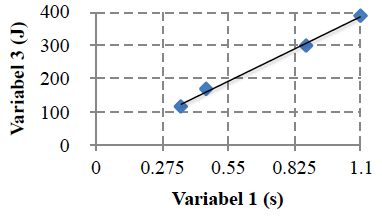
\includegraphics[width=0.6\textwidth]{fig1.png}
  \caption{Exempelfigur som visar variabel 3 som funktion av variabel 1. \label{fvariabel3vs1}}
\end{center}
\end{figure}

\subsection{Underrubrik vid behov}

\subsubsection{Fler underrubriker om så behövs}




%%%%%%%%%%%%%%%%%%%%%%%%%%%%%%%%%%%%%%%%%%%%%%%%%%%%%%%%%%%%%%
% -                      Summary                           - %
%%%%%%%%%%%%%%%%%%%%%%%%%%%%%%%%%%%%%%%%%%%%%%%%%%%%%%%%%%%%%%

\section{Diskussion och slutsatser}

% Kan delas i separata kapitel: ”Diskussion” respektive ”Slutsatser”. Slutsatser skall vara korta och koncisa.
% Ibland är det lämpligast med indelningen ”Diskussion” samt ”Slutsatser och fortsatt arbete”

Här diskuteras (vad betyder/medför) resultaten utifrån ett vidare perspektiv och ställs i relation exempelvis till tidigare arbeten, referera i sådant fall till dessa. Utgående härifrån dras nödvändiga slutsatser som ska svara på de mål som angivits och vad resultaten har för relevans. Koppla slutsatser till uppställda mål.

Diskutera felkällor och osäkerheter.
Det är även lämpligt att i denna del avsluta med förslag och rekommendationer på fortsatta studier och undersökningar i ämnet. Man kan dela upp diskussion, slutsatser och framtida studier i fristående kapitel.




%%%%%%%%%%%%%%%%%%%%%%%%%%%%%%%%%%%%%%%%%%%%%%%%%%%%%%%%%%%%%%
% -                    Bibliography                        - %
%%%%%%%%%%%%%%%%%%%%%%%%%%%%%%%%%%%%%%%%%%%%%%%%%%%%%%%%%%%%%%
\printbibliography % - Here we say that the bibliography should be printed. The section title "References" is printed automatically.

% I denna del anges de källor du använt i ditt arbete. Ange bara de viktigaste och alla
% referenser i listan måste vara refererade till i texten. I referenslistan får det inte
% förekomma någon referens som är ``allmänt bra att ha'' utan endast de referenser som
% författaren själv använt. Alla referenser ska refereras till i texten.
% OBS! använd originalreferenser. Undvik referenser till webbsidor eftersom de kan försvinna/ändras.
% Ett av de vanligaste är att man skriver
% författarnamnet och sedan referensens publikationsår - det s.k. Harvard systemet.
% Exempel: ... även funnet av Charpak (1983)
% Är det två eller flera författare brukar man skriva
% Två författare: ... även funnet av Charpak och Öqvist (1983).
% Flera författare: ... även funnet av Charpak et al. (1983).
% ( et al. är latin (et alii) och betyder ``och andra'').
% Ett annat sätt att ange en referens är att numrera referenserna i den ordning de dyker
% upp i texten och sortera referenslistan i nummerordning.
% Exempel: ... som Öqvist [3] har funnit, och referensen Öqvist dyker då upp som nummer tre i referenslistan.
% En guide för referenser finns här: http://libguides.ltu.se/skrivaoreferera

\end{document}


